\documentclass{article}
\usepackage{listings}
\usepackage{mathrsfs}
\usepackage[utf8]{inputenc}
\usepackage{amssymb}
\usepackage{lipsum}
\usepackage{amsmath}
\usepackage{fancyhdr}
\usepackage{geometry}
\usepackage{scrextend}
\usepackage[english,german]{babel}
\usepackage{titling}
\setlength{\droptitle}{-3cm}
\usepackage{tikz}
\usepackage{algorithm,algpseudocode}
\usepackage[doublespacing]{setspace}
\usetikzlibrary{datavisualization}
\usetikzlibrary{datavisualization.formats.functions}
\usepackage{polynom}
\usepackage{amsmath}
\usepackage{gauss}
\usepackage{tkz-euclide}
\usepackage{minted}
\usetikzlibrary{datavisualization}
\usetikzlibrary{datavisualization.formats.functions}
\author{
Alexander Mattick Kennung: qi69dube\\
Kapitel 1
}
\usepackage{import}
\date{\today}
\geometry{a4paper, margin=2cm}
\usepackage{stackengine}
\parskip 1em
\newcommand\stackequal[2]{%
  \mathrel{\stackunder[2pt]{\stackon[4pt]{=}{$\scriptscriptstyle#1$}}{%
  $\scriptscriptstyle#2$}}
 }
\makeatletter
\renewcommand*\env@matrix[1][*\c@MaxMatrixCols c]{%
  \hskip -\arraycolsep
  \let\@ifnextchar\new@ifnextchar
  \array{#1}}
\makeatother
\lstset{
  language=haskell,
}
\lstnewenvironment{code}{\lstset{language=Haskell,basicstyle=\small}}{}
\usepackage{enumitem}
\setlist{nosep}
\usepackage{titlesec}
\usepackage{ stmaryrd }
\usepackage{verbatim}
\usepackage{tikz-qtree}
\usepackage{bussproofs}

\titlespacing*{\subsection}{0pt}{2pt}{3pt}
\titlespacing*{\section}{0pt}{0pt}{5pt}
\titlespacing*{\subsubsection}{0pt}{1pt}{2pt}
\title{Übung 7}


\begin{document}
	\maketitle
	\[Y=g(X)\]
	(vgl hausaufgabe ``Wurfweite'')\\
	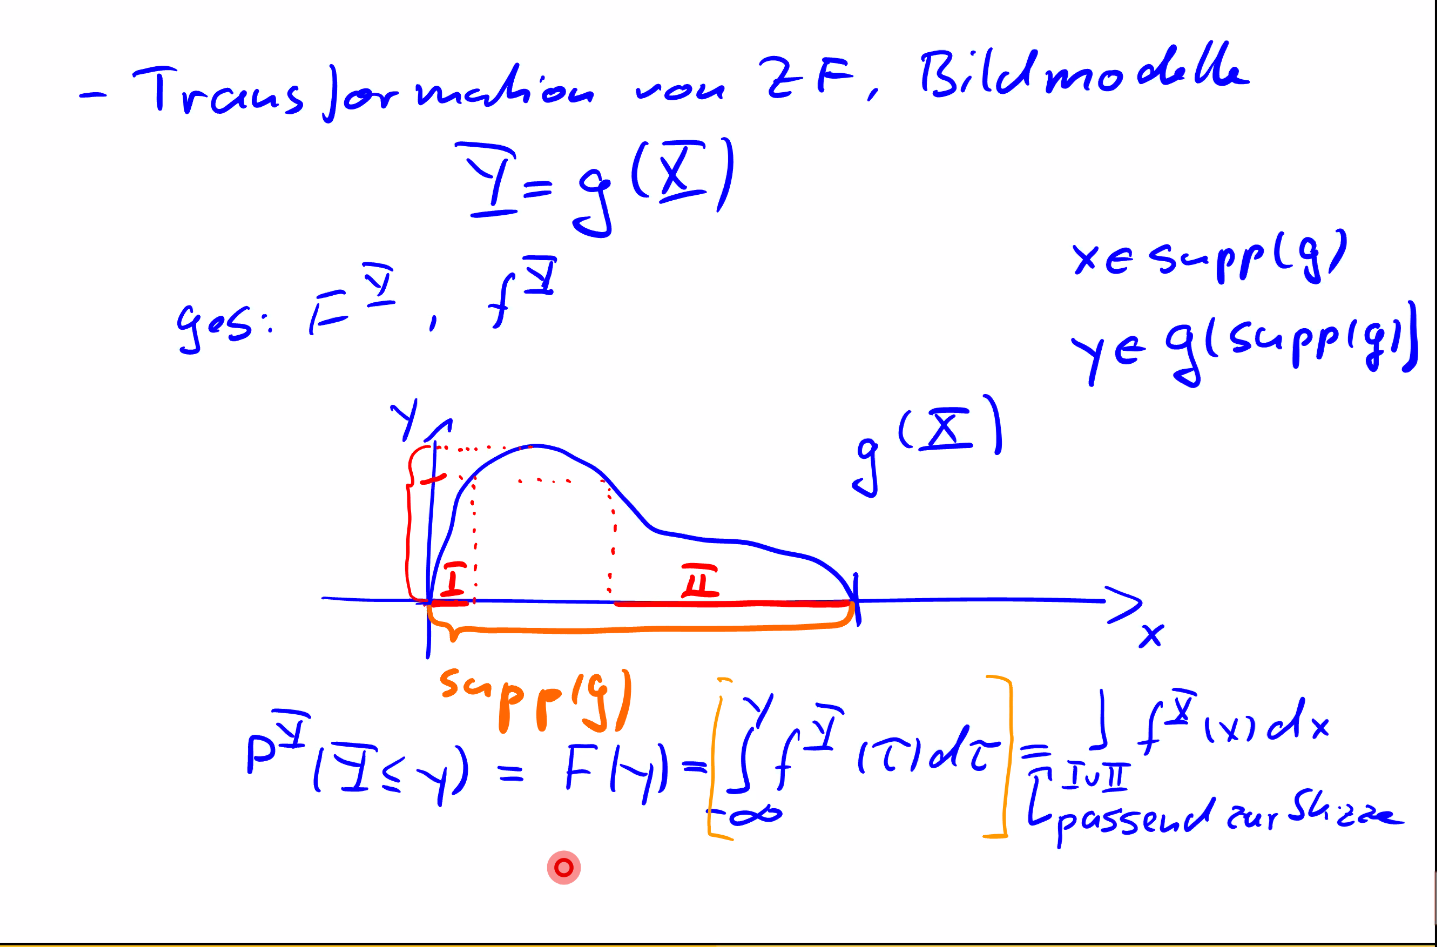
\includegraphics[width=256px]{TransformationVonZV.png}\\
	also Verteilungsfunktion berechnen (weils oft einfacher ist) und dann die dichte durch ableiten bekommen.\\
	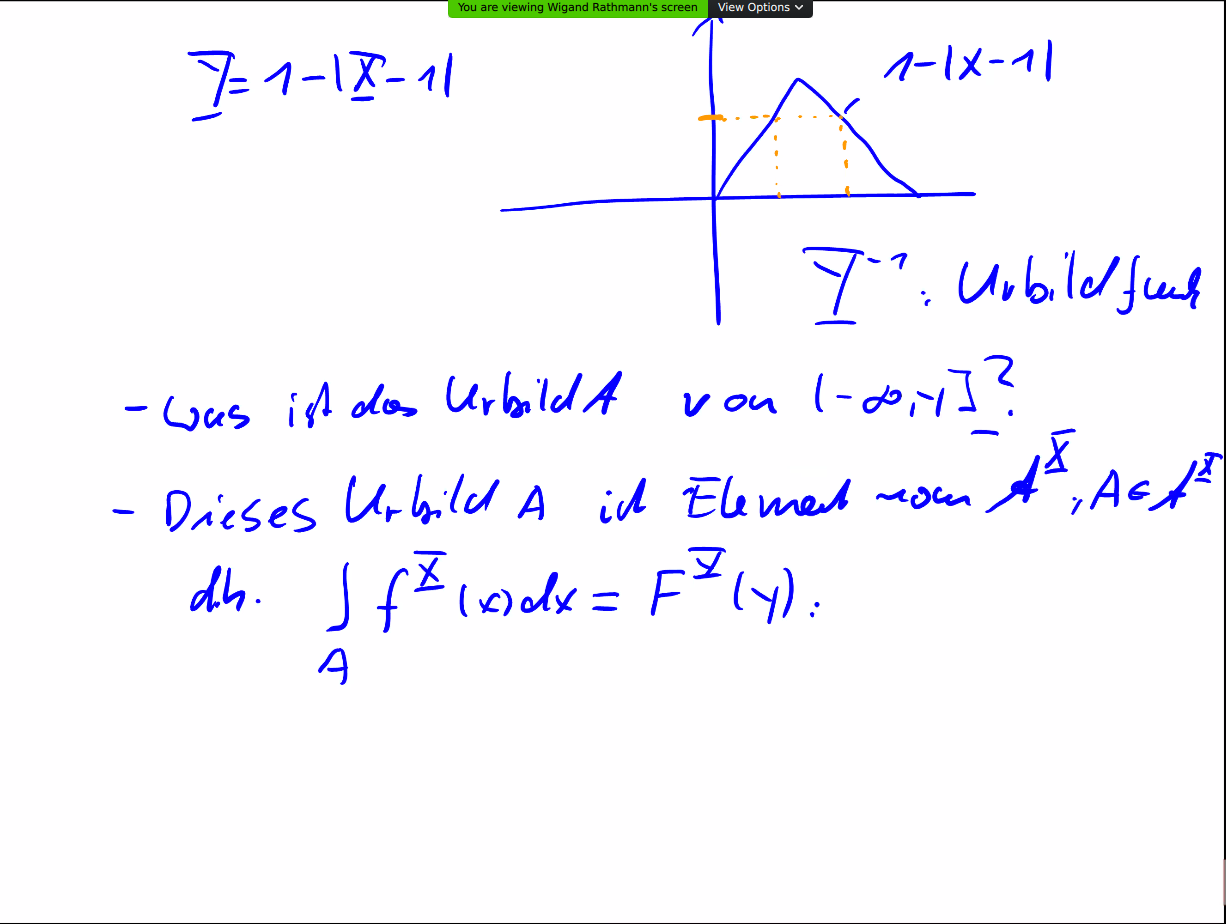
\includegraphics[width=256px]{dreieck.png}\\
	Sprich man schaut sich die Flächen an, die zu werten $y\leq Y$ korrespondieren.\\
	Diese entsprechen dann dem wert von $F^Y(y)$ und kann zu $f^Y(y)$ abgeleitet werden.\\
	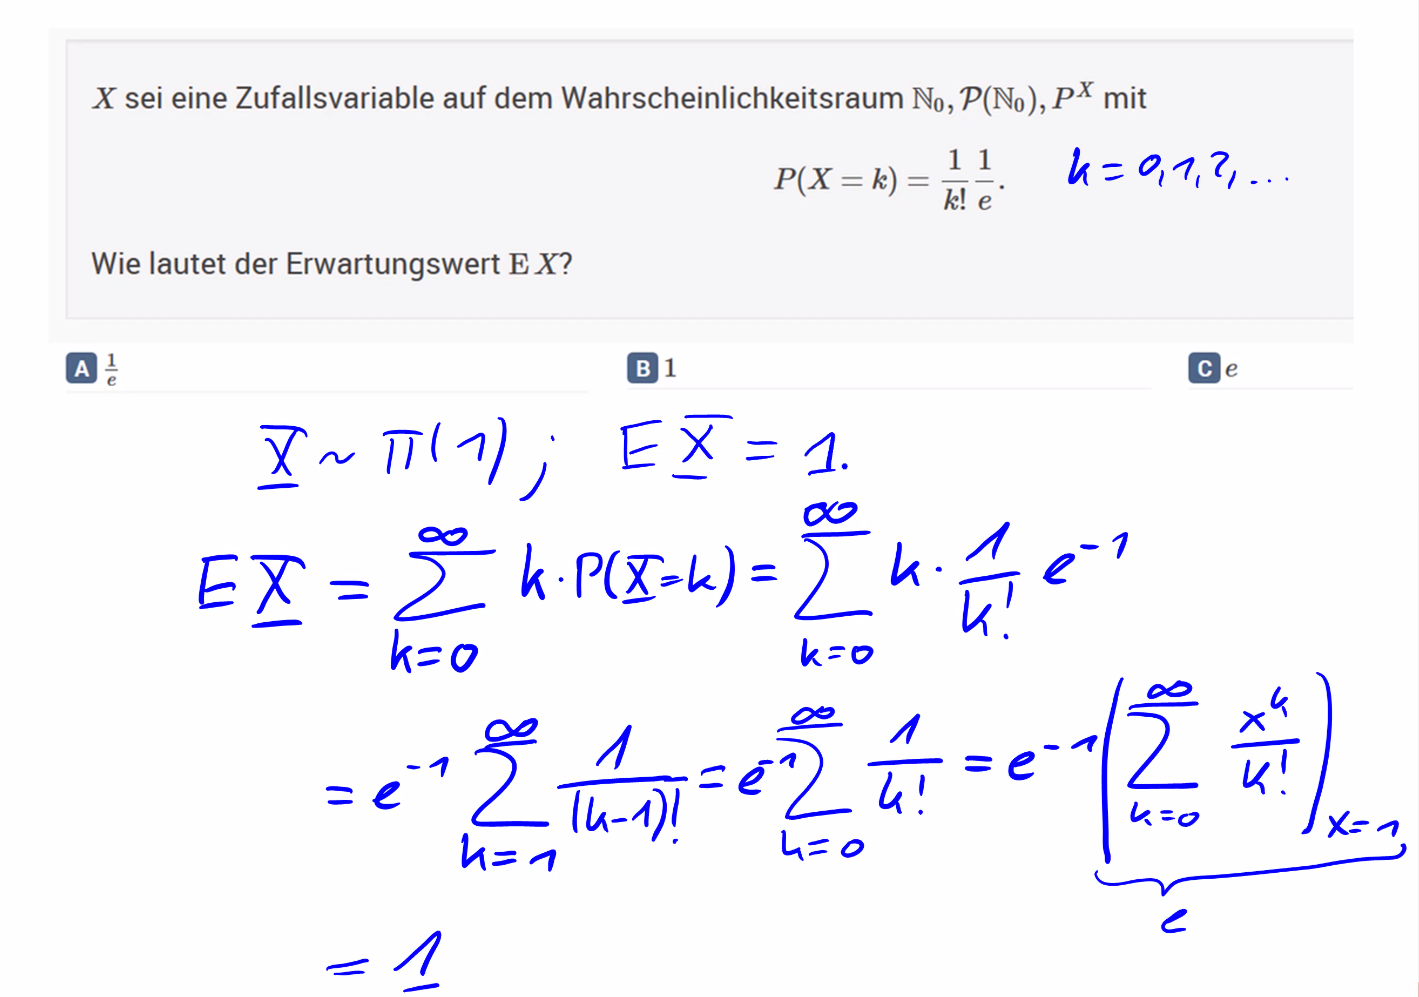
\includegraphics[width=256px]{Poisson-Verteilung.png}\\
	Poisson verteilung $X\sim \pi(1)\implies EX=1$\\
	\\
	\begin{tabular}{c|c|c}
	Name & Erwartung & Var\\
	$x\sim \pi(\lambda)$ &$\lambda$  & $\lambda$ \\
	$x\sim R(a,b)$ &$\frac{a+b}{2}$  & $\frac{(b-a)^2}{12}$  \\
	$x\sim Exp(\lambda)$ & $\frac{1}{\lambda}$ & $\frac{1}{\lambda^2}$ \\
	$x\sim \Gamma_{\alpha,\mu}$ & $\frac{\mu}{\alpha}$  &  $\frac{\mu}{\alpha^2}$\\
	$x\sim N(\mu,\sigma^2)$ & $\mu$ &$\sigma^2$ \\
	$x\sim Nb^0(r,p)$ & $\frac{r(1-p)}{p}$  & $\frac{r(1-p)}{p^2}$\\
	$x\sim Nb^+(r,p)$ &$\frac{r}{p}$  &$\frac{r(1-p)}{p^2}$ \\
	$x\sim B(n,p)$ & $np$& $np(1-p)$\\
	$x\sim B(p)$ & $p$& $p(1-p)$\\
	\end{tabular}
	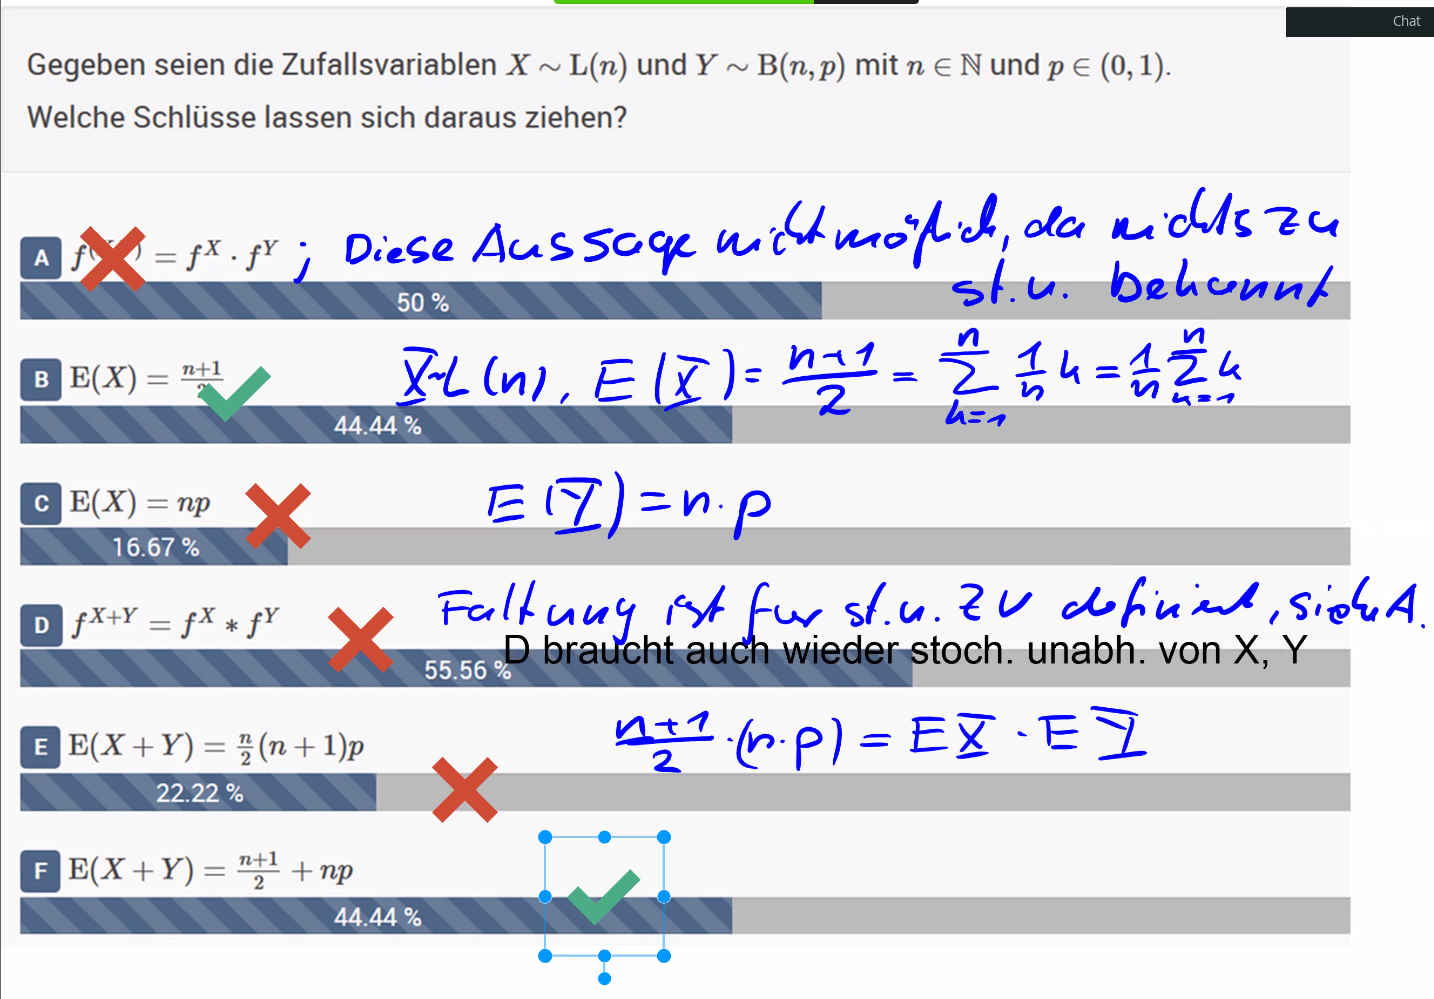
\includegraphics[width=256px]{Fangfragen.png}\\
	Wie wird der Erwartungswert einer ZV Y berechnet, wenn Y eine Funktion anderer YV ist.\\
	Soll heißen $Y=g(X)$\\
	$EY =\int_\mathbb{R} g(x)f^X(x)dx$ (sprich, wir nehmen statt den Wert x, den wert von g der auf y mapped)\\
	$EY =\sum_{x\in\Omega^X} g(x)f^X(x)dx$ (also genau das gleiche).\\
	Wir rechnen also auf das Urbild zurück
	\[EX:=\sum_{k\in\Omega'} kP(X=k)=\sum_{\omega\in\Omega} X(\omega)f(\omega)\]
	wobei $X:\Omega\to\Omega'$ also auf von $\omega$ auf k mapped.\\
	analog bei mehreren stochastisch unabhängigen ZV\\
	Erwartungswert ist monoton $X\leq Y \implies EX\leq EY$ falls $EX,EY$ existieren\\
	c)\\
	linearität
	\[E(aX+b)=aEX+b\]
	Wenn EX und EY existieren, additiv \underline{(auch wenn \textbf{nicht} stochastisch unabhängig!!!!!!!!)}
	\[E(X+Y)=EX+EY\]
	bei \underline{stochastischer unabhängigkeit} gilt
	\[EXY = EX\cdot EY\]
	wenn $EX_i$ existieren für alle i hilt
	\[E(\sum^n_{i=1}X_i)=\sum^n_{i=1}EX_i\]
	Varianz und Streuung
	\[Var X = E(X-EX)^2 = EX^2 -(EX)^2\]
\end{document}